\section{Máximos y Mínimos de Funciones de Varias Variables}

Las derivadas parciales y el gradiente permiten localizar los puntos donde una función alcanza valores extremos. El análisis en varias variables sigue el mismo esquema que en una variable, con la diferencia de que los puntos críticos admiten más tipos de comportamiento local.

Conviene distinguir desde el principio dos nociones. Un extremo \emph{local} compara el valor de la función solo con los puntos cercanos: es el más alto o el más bajo dentro de un entorno pequeño. Un extremo \emph{absoluto} compara con todos los puntos del dominio: es el más alto o el más bajo de toda la región. La siguiente figura muestra la gráfica de una función $f: \mathbb{R}^2 \to \mathbb{R}$ con dos cimas y dos hondonadas de distinta altura, y permite ver ambas ideas sobre la superficie. Un mismo punto puede ser máximo local sin ser el máximo absoluto, pues basta con que exista otra cima más alta en otra parte del dominio.

\begin{center}
\shorthandoff{>}
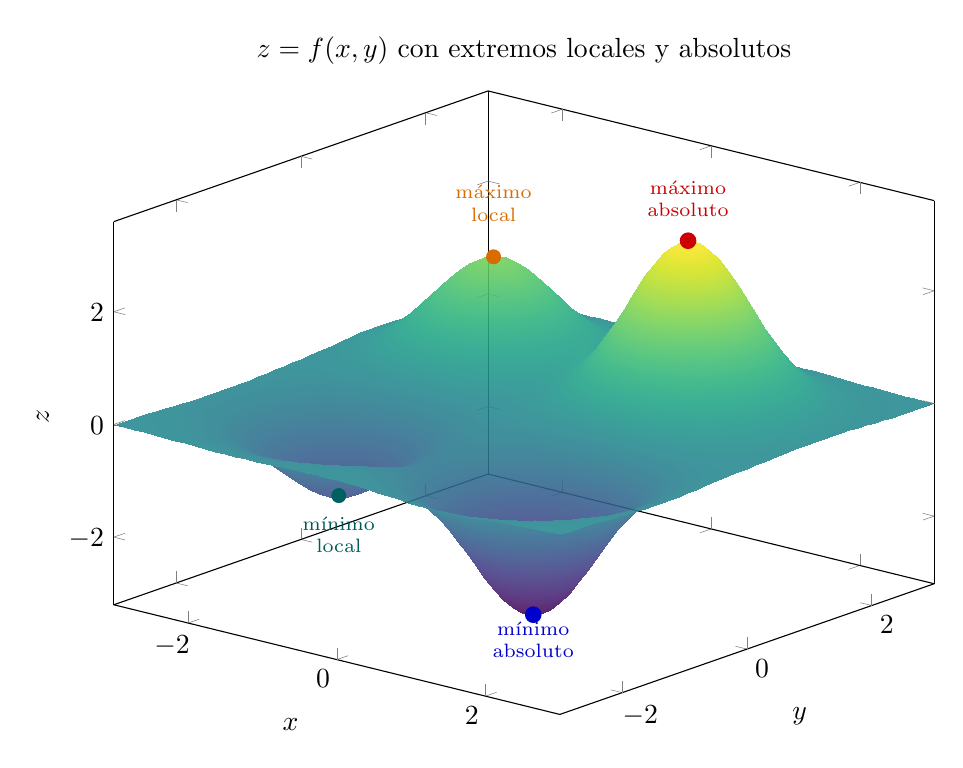
\begin{tikzpicture}
\begin{axis}[
    width=12cm, height=9.5cm,
    view={40}{24},
    colormap/viridis,
    xlabel={$x$}, ylabel={$y$}, zlabel={$z$},
    domain=-3:3, domain y=-3:3,
    samples=45, samples y=45,
    zmin=-3.2, zmax=3.6,
    clip=false,
    title={$z = f(x,y)$ con extremos locales y absolutos},
]
    % Superficie: dos cimas y dos hondonadas de distinta altura
    \addplot3[surf, opacity=0.88, shader=interp, z buffer=sort]
        {3.0*exp(-1.2*((x-1.2)^2+(y-1.2)^2))
         + 1.8*exp(-1.2*((x+1.5)^2+(y-1.3)^2))
         - 2.6*exp(-1.2*((x-1.3)^2+(y+1.4)^2))
         - 1.4*exp(-1.2*((x+1.4)^2+(y+1.3)^2))};
    % Máximo absoluto (cima alta)
    \addplot3[only marks, mark=*, mark size=2.8pt, red!80!black]
        coordinates {(1.2,1.2,3.0)};
    \node at (axis cs:1.2,1.2,3.75) [font=\scriptsize, red!80!black, align=center]
        {máximo\\absoluto};
    % Máximo local (cima baja)
    \addplot3[only marks, mark=*, mark size=2.5pt, orange!85!black]
        coordinates {(-1.5,1.3,1.8)};
    \node at (axis cs:-1.5,1.3,2.75) [font=\scriptsize, orange!85!black, align=center]
        {máximo\\local};
    % Mínimo absoluto (hondonada profunda)
    \addplot3[only marks, mark=*, mark size=2.8pt, blue!80!black]
        coordinates {(1.3,-1.4,-2.6)};
    \node at (axis cs:1.3,-1.4,-3.05) [font=\scriptsize, blue!80!black, align=center]
        {mínimo\\absoluto};
    % Mínimo local (hondonada somera)
    \addplot3[only marks, mark=*, mark size=2.5pt, teal!75!black]
        coordinates {(-1.4,-1.3,-1.4)};
    \node at (axis cs:-1.4,-1.3,-2.1) [font=\scriptsize, teal!70!black, align=center]
        {mínimo\\local};
\end{axis}
\end{tikzpicture}
\end{center}

El máximo absoluto es a la vez un máximo local, pero la cima de la izquierda es solo un máximo local porque existe otra cima más alta. Lo mismo ocurre con las hondonadas: la más profunda da el mínimo absoluto y la otra es solo un mínimo local. En este ejemplo los cuatro extremos son puntos interiores del dominio; cuando la región es cerrada y acotada, los valores extremos también pueden alcanzarse sobre la frontera, situación que se estudia más adelante.

\subsection{Máximos y mínimos locales}

\begin{mydefinition}{Máximo y mínimo local}
Sea $f: D \subseteq \mathbb{R}^2 \to \mathbb{R}$. Se dice que $f$ tiene un máximo local en $(a, b)$ si existe $\delta > 0$ tal que $f(x, y) \leq f(a, b)$ para todo $(x, y) \in D$ con $\|(x,y)-(a,b)\| < \delta$. Análogamente, $f$ tiene un mínimo local en $(a, b)$ si $f(x, y) \geq f(a, b)$ en ese disco. Si la desigualdad vale en todo el dominio $D$, el extremo es absoluto (o global).
\end{mydefinition}

\begin{mytheorem}{Condición necesaria de Fermat}
Si $f$ tiene un extremo local en $(a, b)$ y las derivadas parciales $f_x(a, b)$ y $f_y(a, b)$ existen, entonces:
\[
f_x(a, b) = 0 \qquad \text{y} \qquad f_y(a, b) = 0.
\]
\end{mytheorem}

Los puntos donde $\nabla f = \mathbf{0}$ o donde alguna derivada parcial no existe se llaman puntos críticos de $f$. Todo extremo local es un punto crítico, pero no todo punto crítico es un extremo: puede ser un punto de silla, en el que $f$ crece en unas direcciones y decrece en otras desde ese punto.

\subsection{Criterio de la segunda derivada}

Para clasificar un punto crítico sin necesidad de analizar el signo de $f(x,y)-f(a,b)$ directamente, se utiliza el discriminante formado por las segundas derivadas parciales.

\begin{mytheorem}{Criterio de la segunda derivada}
Sea $f$ con segundas derivadas parciales continuas en una vecindad de $(a, b)$, y suponga que $\nabla f(a, b) = \mathbf{0}$. Define el discriminante:
\[
D(a, b) = f_{xx}(a,b)\,f_{yy}(a,b) - \bigl[f_{xy}(a,b)\bigr]^2.
\]
\begin{itemize}
    \item Si $D > 0$ y $f_{xx}(a,b) > 0$, entonces $(a,b)$ es un mínimo local.
    \item Si $D > 0$ y $f_{xx}(a,b) < 0$, entonces $(a,b)$ es un máximo local.
    \item Si $D < 0$, entonces $(a,b)$ es un punto de silla.
    \item Si $D = 0$, el criterio no concluye y se requiere un análisis adicional.
\end{itemize}
\end{mytheorem}

\textbf{Ejemplo 1.} Sea $f(x, y) = x^2 + y^2 - 4x - 2y + 8$.

Las derivadas parciales son $f_x = 2x - 4$ y $f_y = 2y - 2$. El sistema $f_x = 0$, $f_y = 0$ tiene la solución única $(a, b) = (2, 1)$. Como $f_{xx} = 2$, $f_{yy} = 2$ y $f_{xy} = 0$:
\[
D(2,1) = 2 \cdot 2 - 0^2 = 4 > 0, \qquad f_{xx}(2,1) = 2 > 0.
\]
Por el criterio, $(2, 1)$ es un mínimo local con $f(2, 1) = 3$. Completando el cuadrado, $f(x,y) = (x-2)^2 + (y-1)^2 + 3 \geq 3$, lo que confirma que es el mínimo global.

\begin{center}
\shorthandoff{>}
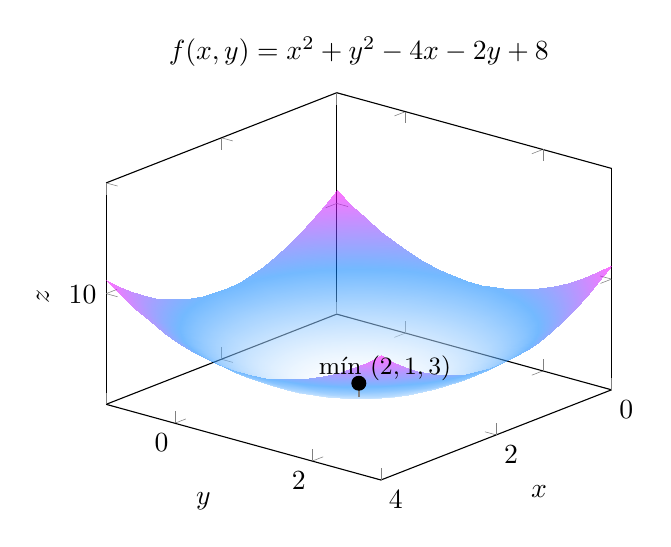
\begin{tikzpicture}
\begin{axis}[
    width=8cm, height=6.5cm,
    view={130}{28},
    colormap/cool,
    xlabel={$x$}, ylabel={$y$}, zlabel={$z$},
    zmin=2, zmax=18,
    domain=0:4, domain y=-1:3,
    samples=20, samples y=20,
    clip=false,
    title={$f(x,y)=x^2+y^2-4x-2y+8$},
]
    \addplot3[surf, opacity=0.55, shader=interp]
        {x^2 + y^2 - 4*x - 2*y + 8};
    \addplot3[only marks, mark=*, mark size=2.5pt, black]
        coordinates {(2,1,3)};
    \node at (axis cs:2.5,1.8,6) [font=\small] {mín $(2,1,3)$};
    \addplot3[dashed, gray, thick] coordinates {(2,1,2) (2,1,3)};
\end{axis}
\end{tikzpicture}
\end{center}

\textbf{Ejemplo 2.} Sea $f(x, y) = x^3 + y^3 - 3xy$.

De $f_x = 3x^2 - 3y = 0$ se obtiene $y = x^2$; sustituyendo en $f_y = 3y^2 - 3x = 0$ resulta $3x^4 - 3x = 3x(x^3-1) = 0$, con soluciones $x = 0$ y $x = 1$.

Los puntos críticos son $(0, 0)$ y $(1, 1)$. Las segundas derivadas son $f_{xx} = 6x$, $f_{yy} = 6y$ y $f_{xy} = -3$.

En $(0, 0)$: $D = (0)(0) - (-3)^2 = -9 < 0$, de modo que $(0, 0)$ es un punto de silla, con $f(0,0) = 0$.

En $(1, 1)$: $D = (6)(6) - (-3)^2 = 27 > 0$ y $f_{xx}(1,1) = 6 > 0$, de modo que $(1, 1)$ es un mínimo local, con $f(1,1) = 1 + 1 - 3 = -1$.

\begin{center}
\shorthandoff{>}
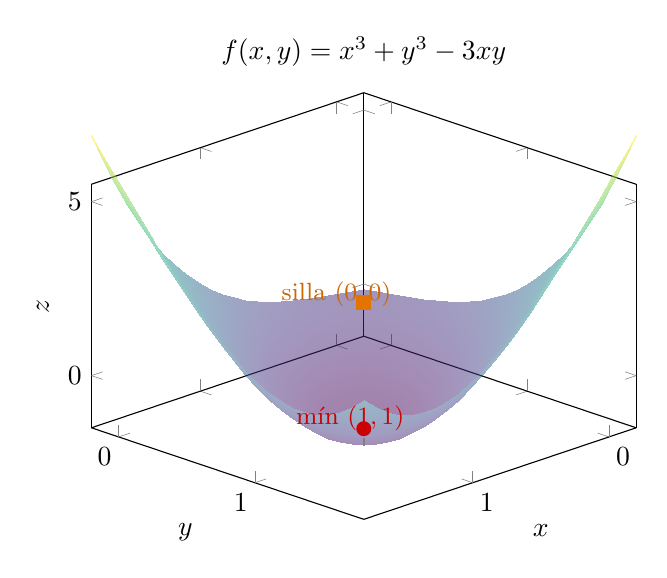
\begin{tikzpicture}
\begin{axis}[
    width=8.5cm, height=7cm,
    view={135}{28},
    colormap/viridis,
    xlabel={$x$}, ylabel={$y$}, zlabel={$z$},
    zmin=-1.5, zmax=5.5,
    domain=-0.2:1.8, domain y=-0.2:1.8,
    samples=24, samples y=24,
    clip=false,
    title={$f(x,y)=x^3+y^3-3xy$},
]
    \addplot3[surf, opacity=0.50, shader=interp]
        {x^3 + y^3 - 3*x*y};
    % Saddle at (0,0,0)
    \addplot3[only marks, mark=square*, mark size=2.5pt, orange!90!black]
        coordinates {(0,0,0)};
    \node at (axis cs:0.35,0.15,0.9) [font=\small, orange!80!black] {silla $(0,0)$};
    % Min at (1,1,-1)
    \addplot3[only marks, mark=*, mark size=2.5pt, red!80!black]
        coordinates {(1,1,-1)};
    \node at (axis cs:1.35,1.25,0.1) [font=\small, red!80!black] {mín $(1,1)$};
    % Dashed vertical to min
    \addplot3[dashed, gray, thick] coordinates {(1,1,-1.5) (1,1,-1)};
\end{axis}
\end{tikzpicture}
\end{center}

\subsection{Máximos y mínimos absolutos en una región $D$}

\begin{mytheorem}{Teorema de valores extremos}
Si $f$ es continua en un conjunto $D \subseteq \mathbb{R}^2$ cerrado y acotado, entonces $f$ alcanza un máximo absoluto y un mínimo absoluto en $D$.
\end{mytheorem}

Para hallar los extremos absolutos de $f$ en $D$ se aplica el siguiente procedimiento:
\begin{enumerate}
    \item Calcular los valores de $f$ en todos los puntos críticos del interior de $D$.
    \item Encontrar los valores extremos de $f$ restringida a la frontera $\partial D$.
\end{enumerate}
El mayor de todos los valores obtenidos es el máximo absoluto; el menor, el mínimo absoluto.

\textbf{Ejemplo 3.} Encuentre los extremos absolutos de $f(x, y) = x^2 + y^2 - 2x$ en el disco cerrado $D: x^2 + y^2 \leq 4$.

\textit{Puntos críticos interiores.} De $f_x = 2x - 2 = 0$ y $f_y = 2y = 0$ se obtiene $(1, 0)$. Como $1^2 + 0^2 = 1 < 4$, el punto es interior a $D$, con $f(1, 0) = 1 - 2 = -1$.

\textit{Frontera.} Parametrizando la circunferencia $x^2 + y^2 = 4$ con $x = 2\cos t$, $y = 2\sin t$:
\[
g(t) = 4\cos^2 t + 4\sin^2 t - 4\cos t = 4 - 4\cos t.
\]
De $g'(t) = 4\sin t = 0$ se obtienen $t = 0$ y $t = \pi$, con puntos $(2, 0)$ y $(-2, 0)$:
\[
f(2, 0) = 4 - 4 = 0, \qquad f(-2, 0) = 4 + 4 = 8.
\]

Comparando todos los candidatos: el mínimo absoluto es $-1$, alcanzado en $(1, 0)$; el máximo absoluto es $8$, alcanzado en $(-2, 0)$.

\begin{center}
\shorthandoff{>}
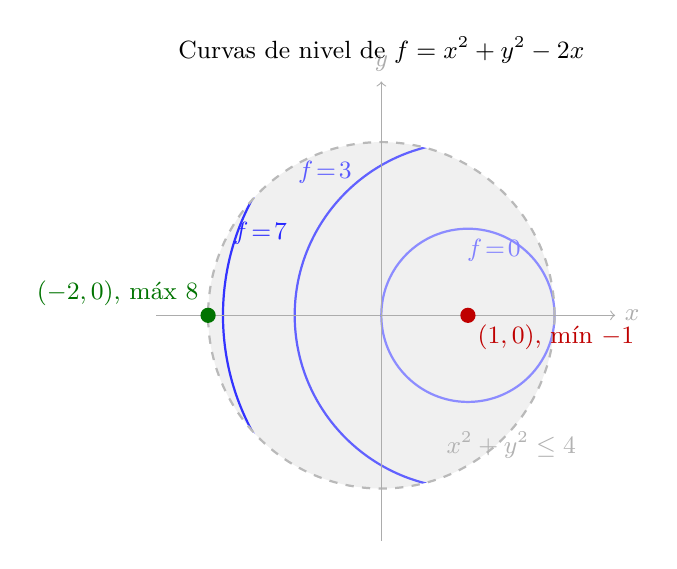
\begin{tikzpicture}[scale=1.1, every node/.style={font=\small}]
    % Shaded disk
    \fill[gray!12] (0,0) circle (2);
    % Level curve c=0: (x-1)^2+y^2=1, center (1,0) r=1
    \draw[blue!45, thick] (1,0) circle (1);
    % Level curve c=3: (x-1)^2+y^2=4, center (1,0) r=2 — clip to disk
    \begin{scope}
        \clip (0,0) circle (2);
        \draw[blue!62, thick] (1,0) circle (2);
    \end{scope}
    % Level curve c=7: (x-1)^2+y^2=8, r=2.828 — clip to disk
    \begin{scope}
        \clip (0,0) circle (2);
        \draw[blue!80, thick] (1,0) circle (2.828);
    \end{scope}
    % Boundary of disk
    \draw[gray!55, thick, dashed] (0,0) circle (2);
    % Level labels
    \node[blue!50] at (1.3, 0.75) {$f\!=\!0$};
    \node[blue!65] at (-0.65, 1.65) {$f\!=\!3$};
    \node[blue!85] at (-1.4, 0.95) {$f\!=\!7$};
    % Axes
    \draw[->, gray!65] (-2.6,0) -- (2.7,0) node[right] {$x$};
    \draw[->, gray!65] (0,-2.6) -- (0,2.7) node[above] {$y$};
    % Min point (1,0), f=-1
    \fill[red!75!black] (1,0) circle (2.5pt);
    \node[below right, red!75!black] at (1,0) {$(1,0)$, mín $-1$};
    % Max point (-2,0), f=8
    \fill[green!45!black] (-2,0) circle (2.5pt);
    \node[above left, green!45!black] at (-2,0) {$(-2,0)$, máx $8$};
    % Disk label
    \node[gray!60] at (1.5,-1.5) {$x^2+y^2\le 4$};
    % Title
    \node[above] at (0,2.8) {Curvas de nivel de $f = x^2+y^2-2x$};
\end{tikzpicture}
\end{center}

\subsection{Ejercicios}

\begin{enumerate}
    \item Encuentre y clasifique todos los puntos críticos de $f(x, y) = x^3 - 3x + y^2 - 2y + 5$.

    \item Encuentre y clasifique todos los puntos críticos de $f(x, y) = x^2 + xy + y^2 - 3x$.

    \item Sea $f(x, y) = x^3 + y^3 - 3x^2 - 3y^2 + 4$.
\begin{enumerate}
    \item Encuentre todos los puntos críticos de $f$.
    \item Clasifique cada uno usando el criterio de la segunda derivada.
    \item Calcule el valor de $f$ en cada extremo local y determine si alguno de ellos es absoluto.
\end{enumerate}

    \item Sea $f(x, y) = x^4 + y^4 - 4xy$.
\begin{enumerate}
    \item Determine todos los puntos críticos de $f$.
    \item Clasifíquelos con el criterio de la segunda derivada y calcule el valor de $f$ en cada mínimo local.
    \item Justifique que $f$ no tiene máximo absoluto en $\mathbb{R}^2$.
\end{enumerate}

    \item Encuentre los extremos absolutos de $f(x, y) = 2x + 3y$ en el disco cerrado $D: x^2 + y^2 \leq 4$.

    \item Encuentre los extremos absolutos de $f(x, y) = xy$ en la región triangular $D$ con vértices $(0, 0)$, $(4, 0)$ y $(0, 4)$.

    \item Sea $f(x, y) = ax^2 + bxy + cy^2$ con $a > 0$ y $4ac - b^2 > 0$.
\begin{enumerate}
    \item Muestre que $(0, 0)$ es el único punto crítico de $f$.
    \item Use el criterio de la segunda derivada para clasificarlo.
    \item Deduzca que $f(x, y) > 0$ para todo $(x, y) \neq (0, 0)$ y que el mínimo absoluto de $f$ en $\mathbb{R}^2$ es $f(0, 0) = 0$.
\end{enumerate}

    \item Encuentre los extremos absolutos de $f(x, y) = x^2 + xy + y^2$ en el disco cerrado $D: x^2 + y^2 \leq 1$.
\begin{enumerate}
    \item Analice los puntos críticos en el interior de $D$.
    \item Parametrice la frontera $x^2 + y^2 = 1$ y determine los extremos de $f$ sobre ella.
    \item Concluya cuáles son el mínimo y el máximo absolutos y en qué puntos se alcanzan.
\end{enumerate}

\end{enumerate}
